\section{The Omega Holographic Principle: From Spiral to Horizon}

\begin{figure}[ht]
\centering
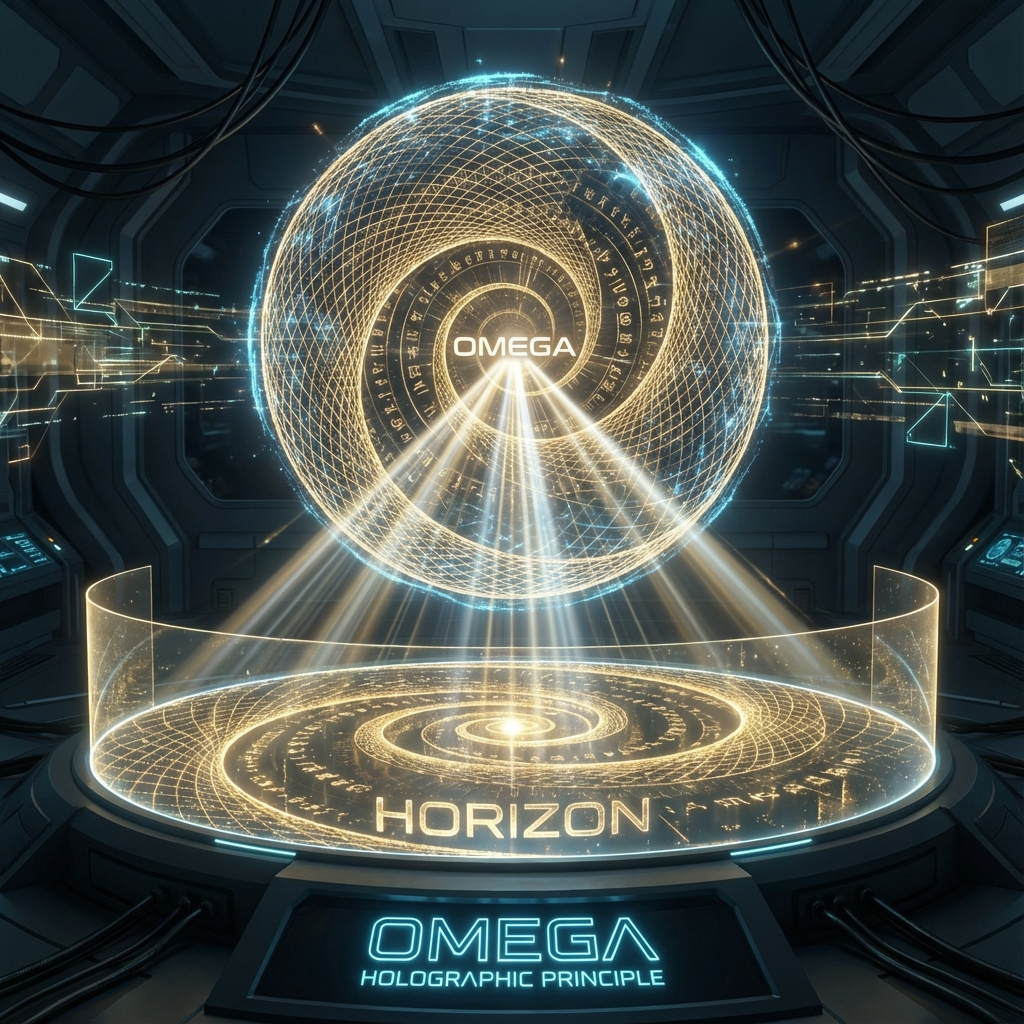
\includegraphics[width=0.8\textwidth]{assets/chapter09-04-omega-holographic-principle.png}
\caption{Omega Holographic Principle}
\end{figure}

In standard physics, the Holographic Principle is usually introduced as an axiom or conjecture to explain the area law of black hole entropy ($S = A/4 l_P^2$). Although theories like AdS/CFT duality have achieved great mathematical success, mainstream physics lacks a fundamental geometric explanation for \textbf{``why''} the universe has this holographic property---i.e., why information in three-dimensional volume can be losslessly encoded on a two-dimensional boundary.

Based on the \textbf{Omega Equivalence Principle} established in the previous section (vector $\cong$ sphere $\cong$ spiral), we no longer need to assume the holographic principle but can construct it directly as a \textbf{geometric theorem}. This section will prove: the holographic horizon is not a physical boundary wall of three-dimensional space but the \textbf{projection of the ``scanning trajectory'' left by the Fibonacci spiral on the Hilbert space sphere}.

\subsection{Projective Geometry and Horizon Generation}

According to the Omega Equivalence Principle, the universe's ontology is a high-dimensional unit hypersphere $S^{\infty}$ (defined by the normalization condition of $|\Omega\rangle$). However, as internal observers, we cannot directly see the entirety of this sphere (that is the God's-eye view). The physical reality we perceive is the \textbf{Tangent Point} and its historical trajectory as the evolution operator $\hat{U}_g(\tau)$ moves on the sphere.

This introduces the perspective of \textbf{Projective Geometry}.
The physical state space of quantum mechanics is actually \textbf{Complex Projective Space} $\mathbb{CP}^{\infty}$.
\[|\psi\rangle \sim e^{i\theta} |\psi\rangle\]
This means that each physical state corresponds to a \textbf{Ray} passing through the origin.

\textbf{The Construction Process of Horizon}:
\begin{enumerate}
\item \textbf{Light Source}: The center (truth/Omega point).
\item \textbf{Trajectory}: The Fibonacci spiral line, representing the evolutionary history of intrinsic time $\tau$.
\item \textbf{Screen}: When we intercept a certain moment $\tau_{now}$ of the universe, we are actually defining a tangent plane orthogonal to the current spiral position.
\end{enumerate}

\begin{figure}[ht]
\centering
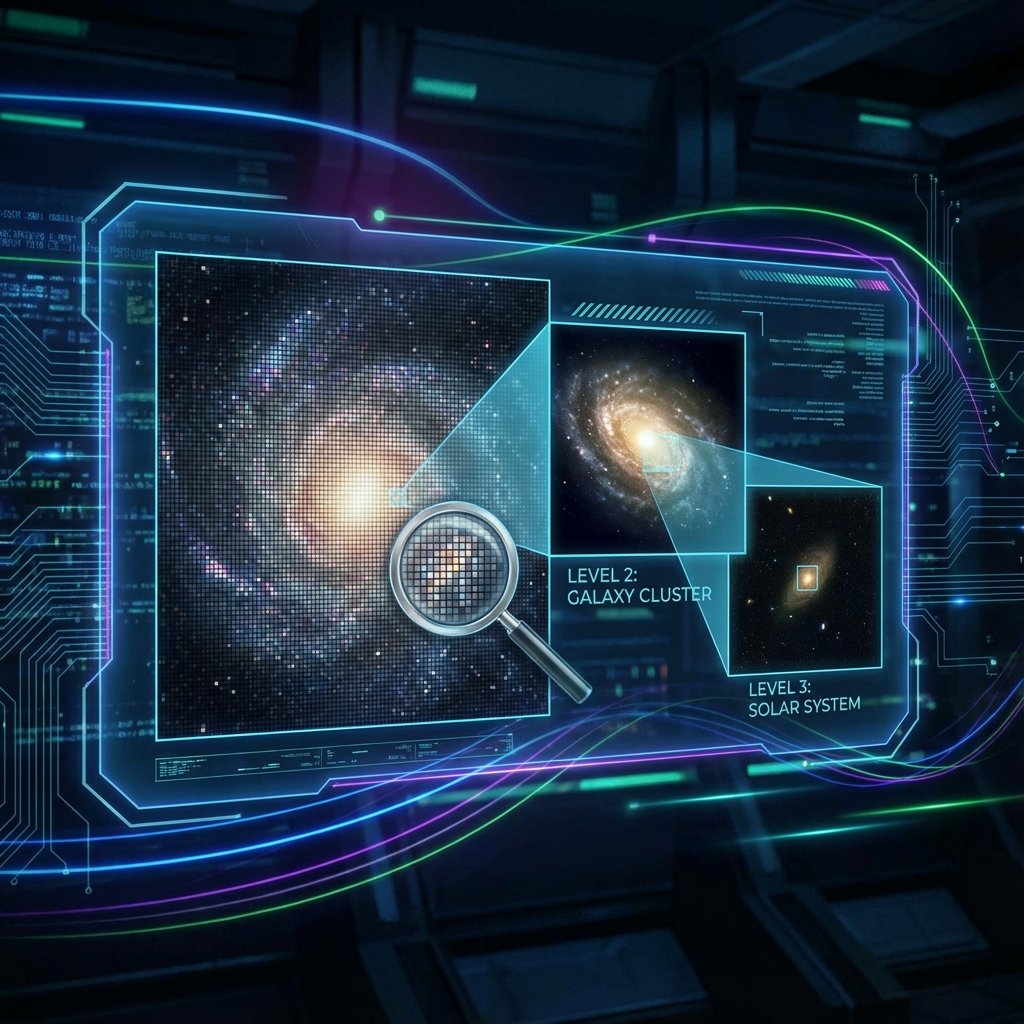
\includegraphics[width=0.8\textwidth]{assets/chapter09-04-holographic-pixel-universe.png}
\caption{Holographic Pixel Universe}
\end{figure}

In this geometric construction, the so-called ``holographic horizon'' is the \textbf{sum of projections of all past spiral trajectories on the current tangent plane}. The horizon is not a skin wrapping a box; it is the \textbf{Topological Projection} of history in the present.

\subsection{Geometric Derivation of the Area Law}

Now let us derive the famous area law $N \propto A$.
In Omega Theory, information quantity $N$ is essentially the discrete number of evolution steps (i.e., the integer count of $\tau$).
Holographic area $A$ is the \textbf{Covered Area} swept by the spiral line on the phase space sphere.

Examining the geometric properties of the Fibonacci spiral. On the unit sphere, the spiral point set generated by the golden angle $\theta_g$ has the property of \textbf{Weyl Equidistribution}. This means the spiral line will not be dense here and sparse there but uniformly fills the sphere with constant density.

Let $\sigma$ be the characteristic micro-area occupied by a single Omega cell (one time step) on the phase space sphere (equivalent to a ``Planck pixel'').
\[d A = \sigma \cdot d \tau\]

Integrating over intrinsic time, we get the total covered area:
\[A(\tau) = \int_0^\tau \sigma dt = \sigma \cdot \tau\]

Since the total information quantity (number of bits) $N(\tau)$ is proportional to the number of time steps $\tau$ (according to Section 9.1), we immediately obtain the core equation of the holographic principle:
\[N(\tau) \propto \frac{A(\tau)}{\sigma} \sim \frac{A}{l_P^2}\]

\textbf{Physical Interpretation}:
This shows that the essence of the holographic principle is not ``three-dimensional space encoded on a two-dimensional surface'' but \textbf{``one-dimensional time sequence (spiral) compactly wound on a two-dimensional manifold (sphere)''}.

\begin{itemize}
\item \textbf{The area $A$ we see}: Actually the \textbf{curling of time}. Space is the accumulation of time.
\item \textbf{The volume $V$ we perceive}: Is the holographic reconstruction illusion of area.
\end{itemize}

\subsection{Bekenstein-Fibonacci Bound}

Based on this, we can revise the traditional Bekenstein bound and propose a more precise \textbf{Bekenstein-Fibonacci Bound}.

In standard holographic theory, maximum entropy $S_{max} = A / 4l_P^2$. The coefficient $1/4$ is usually derived from black hole thermodynamics.
In the Omega construction, due to the non-ergodicity of the spiral, phase space is not a continuous surface but a discrete lattice. The arrangement efficiency of these lattices is controlled by the \textbf{Golden Ratio $\phi$}.

\textbf{Theorem 9.4 (Omega Holographic Theorem)}:
The maximum information quantity $I_{max}$ that any causally closed region (causal diamond) can contain is strictly equal to the number of Fibonacci spiral steps $N_{\phi}$ required to generate the boundary geometry of that region.
The numerical relationship is:
\[I_{max} = \frac{A_{\Omega}}{\sigma_{\phi}} = \frac{\text{Projected Area}}{\text{Golden Pixel Area}}\]
where $\sigma_{\phi}$ is the minimum geometric coherence unit defined by $\phi$.

This means that the universe's information storage efficiency is \textbf{optimal}. Any attempt to store more information per unit area than $\phi$-tiling (i.e., compression beyond golden density) will cause \textbf{Self-intersection} of spiral trajectories. Physically, this trajectory overlap manifests as \textbf{gravitational collapse}, forming black holes. The black hole horizon is essentially a historical deadlock where spiral trajectories overlap excessively and can no longer be resolved as a single path.

\subsection{Conclusion: Holography as Memory}

The holographic principle constructed through the Omega Equivalence Principle reveals a profound ontological fact:
\textbf{The holographic screen is not a spatial boundary but a slice of memory.}

When we look up at the starry sky and see that vast celestial sphere (holographic screen), we are not seeing a distant physical entity; we are seeing the \textbf{projection of all computational history} accumulated from the Big Bang (spiral starting point) to this moment (spiral tangent point).
The universe is holographic because it has never lost any computational step. All the past is laid out at the edge of the present in the form of \textbf{geometric area}. Every square centimeter of the horizon is inscribed with an instant from billions of years ago.
